\section{Программная реализация}

Весь проект реализован с использованием языка программирования Python. Программная реализация состоит из трёх частей:
\begin{enumerate}
\item 
Модуль classifiers содержит классы и функции для работы с
алгоритмами классификации, для выбора признаков,
перекрёстной проверки, а также для работы с корпусами данных.

\item 
Модуль twitter\_api\_wrapper содержит класс-обёртку для 
доступа Twitter API. Использует библиотеку python-oauth2.

\item 
Веб-приложение twitter\_sentiment служит для поиска
мнений в социальной сети Twitter. Веб-приложение написано на Django.
\end{enumerate}

\subsection{Модуль classifiers}
\begin{figure}[!ht]
\begin{center}
\includesvg[]{../resources/uml/diagram_test.svg}
\caption{Диаграмма классов для классификаторов}
\label{gr:test}
\end{center}
\end{figure} 

\subsection{Модуль classifiers}
\begin{figure}[!ht]
\begin{center}
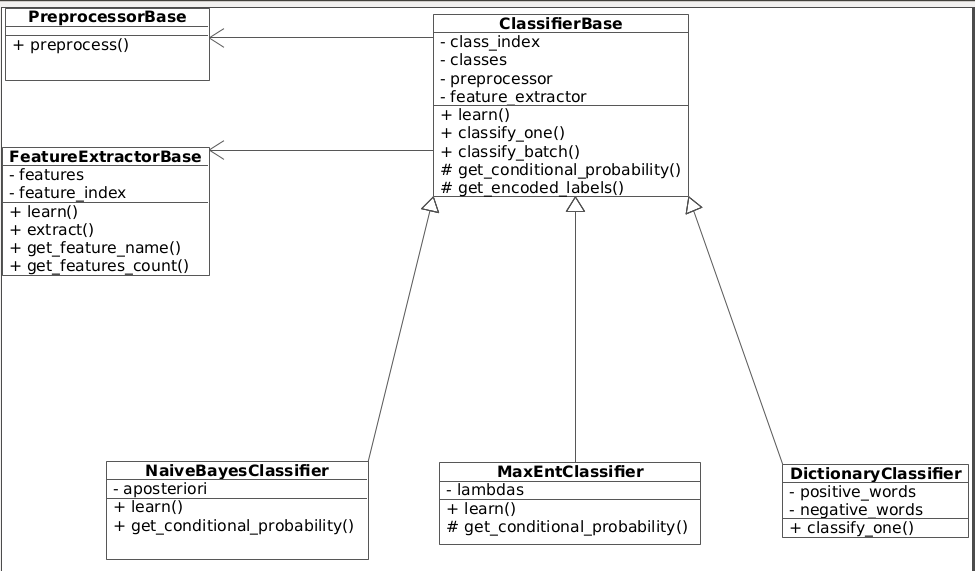
\includegraphics[scale=0.4, trim=0mm 0mm 0mm 0mm, clip]{../resources/uml/diag1.png}
\caption{Диаграмма классов для классификаторов}
\label{gr:classifiers}
\end{center}
\end{figure} 

\begin{figure}[!Ht]
\begin{center}
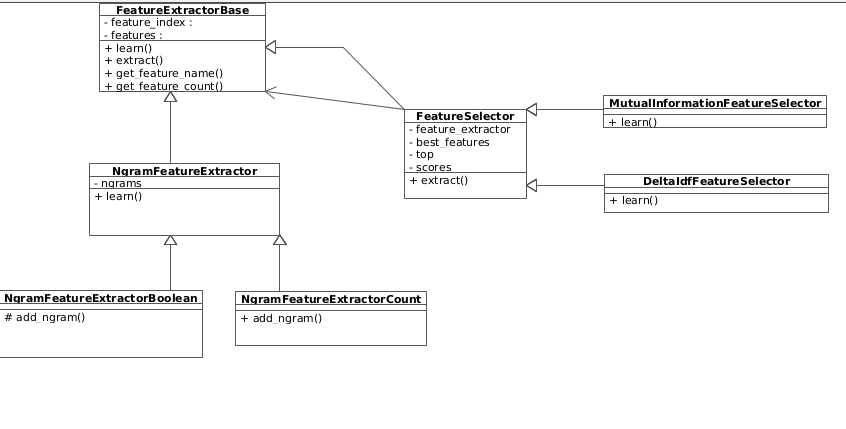
\includegraphics[scale=0.4, trim=0mm 0mm 0mm 0mm, clip]{../resources/uml/diag2.png}
\caption{Диаграмма классов для feature\_extractor'ов}
\label{gr:extractors}
\end{center}
\end{figure} 

\newpage
\subsection{Веб-приложение}
Веб-приложение было разработано при помощи веб-фреймворка Django.
Интерфейс разработан с помощи css-фреймворка ZURB Foundation.

На главной странице пользователь может ввести название
сущности, интересующей его. 
\begin{figure}[!ht]
\begin{center}
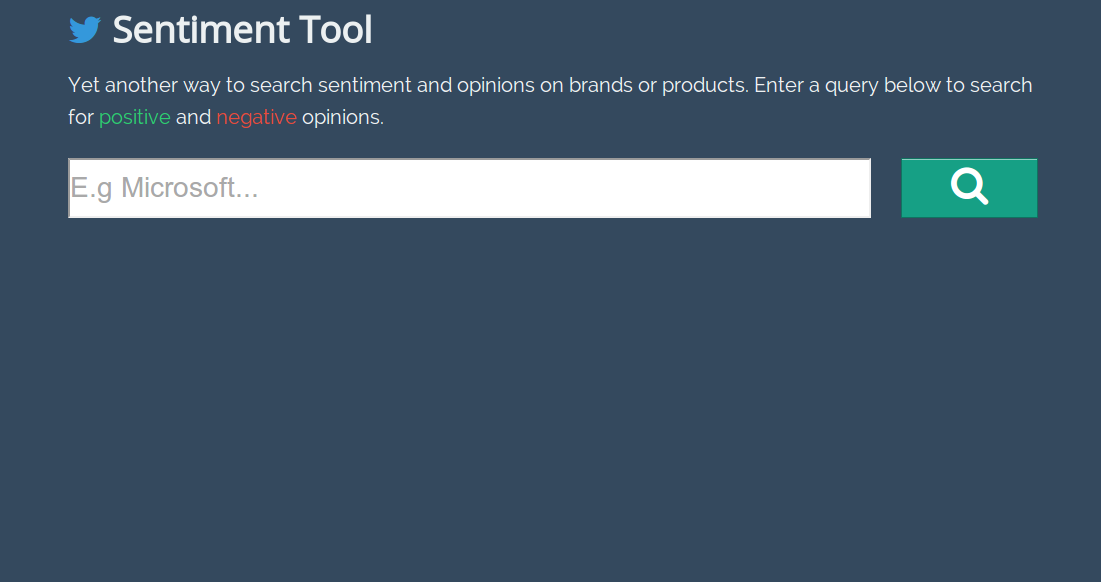
\includegraphics[scale=0.4, trim=0mm 0mm 0mm 0mm, clip]{../resources/screens/1.png}
\caption{Главная страница приложения}
\label{gr:mainpage}
\end{center}
\end{figure} 


После того, как пользователь кликнул на кнопку поиска, происходит ajax-запрос
к серверу. Сервер возвращает уже классифицированные сообщения в 
формате JSON. По умолчанию показываются последние 400 сообщений.
Сообщения, имеющие отрицательную тональность подсвечены красным, положительную --- зелёным, нейтральную --- тёмно-синим.
\begin{figure}[!ht]
\begin{center}
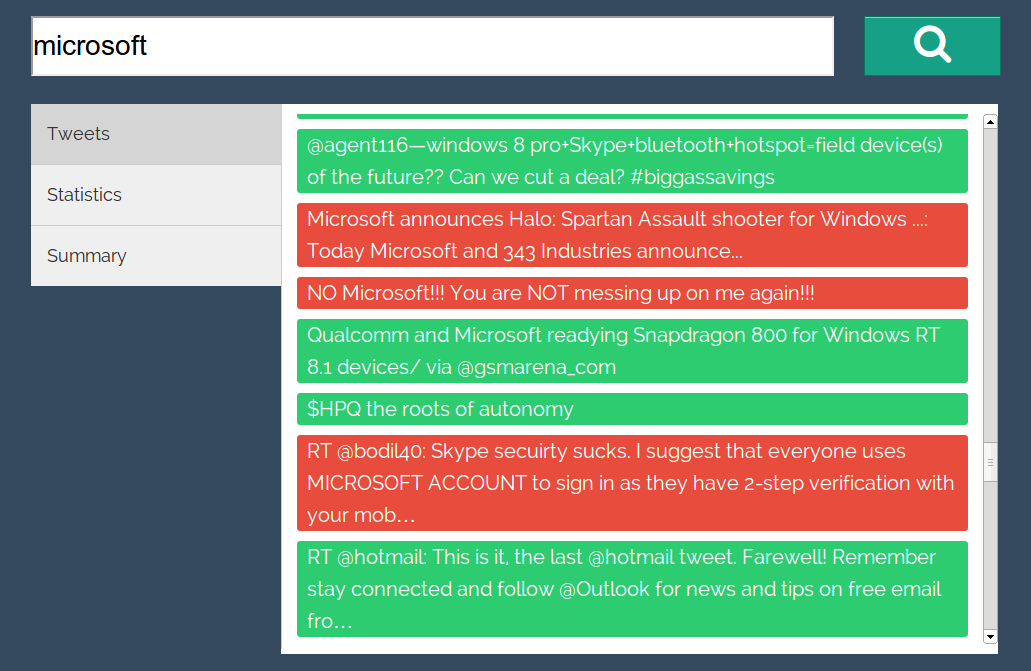
\includegraphics[scale=0.4, trim=0mm 0mm 0mm 0mm, clip]{../resources/screens/2.png}
\caption{Вкладка сообщений}
\label{gr:messages}
\end{center}
\end{figure} 

На вкладке ``Statistics'' (статистика) отображается количество сообщений каждой категории,
а также круговая диаграмма для того, чтобы быстро оценить общее мнение
об объекте поиска.
\begin{figure}[!ht]
\begin{center}
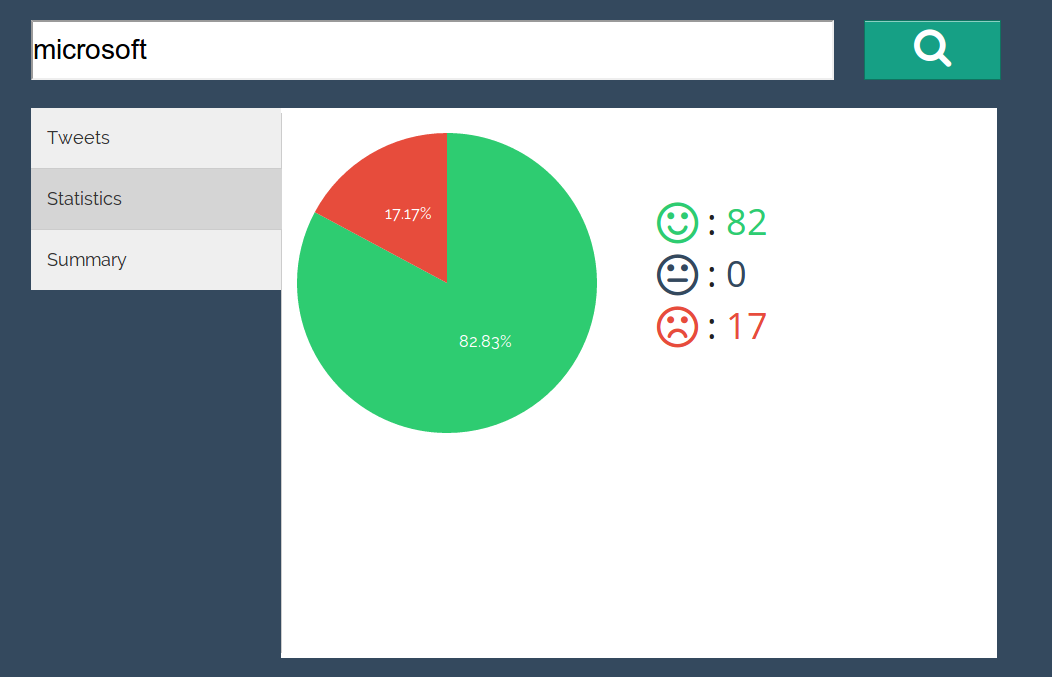
\includegraphics[scale=0.4, trim=0mm 0mm 0mm 0mm, clip]{../resources/screens/3.png}
\caption{Вкладка статистики}
\label{gr:stats}
\end{center}
\end{figure} 


На вкладке ``Summary'' (сводка) отображаются два облака слов --- положительное 
(популярные слова, употребляющиеся в позитивном контексте) и отрицательное.
Размер слова пропорционален логарифму частоты употребления.
\begin{figure}[!ht]
\begin{center}
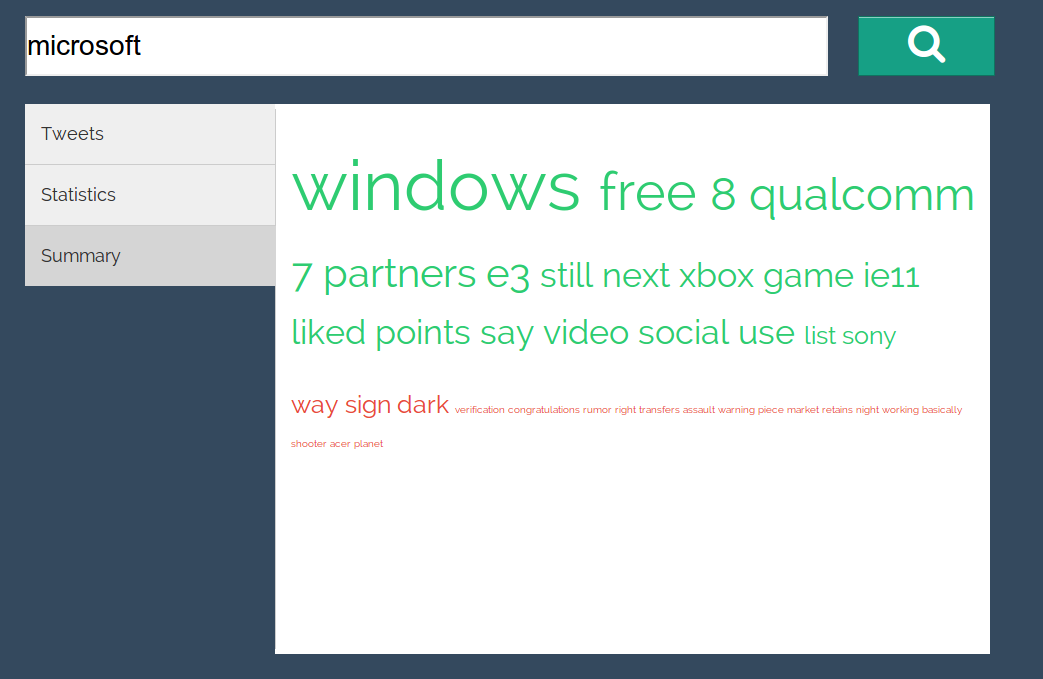
\includegraphics[scale=0.4, trim=0mm 0mm 0mm 0mm, clip]{../resources/screens/4.png}
\caption{Вкладка сводки}
\label{gr:summary}
\end{center}
\end{figure} 